%-----------------------------------------------------------------------
\subsection{Train Supervision}
%-----------------------------------------------------------------------
%\tbc
%Group 1 (Christian Stahl)

\begin{figure}[!h]
\centering
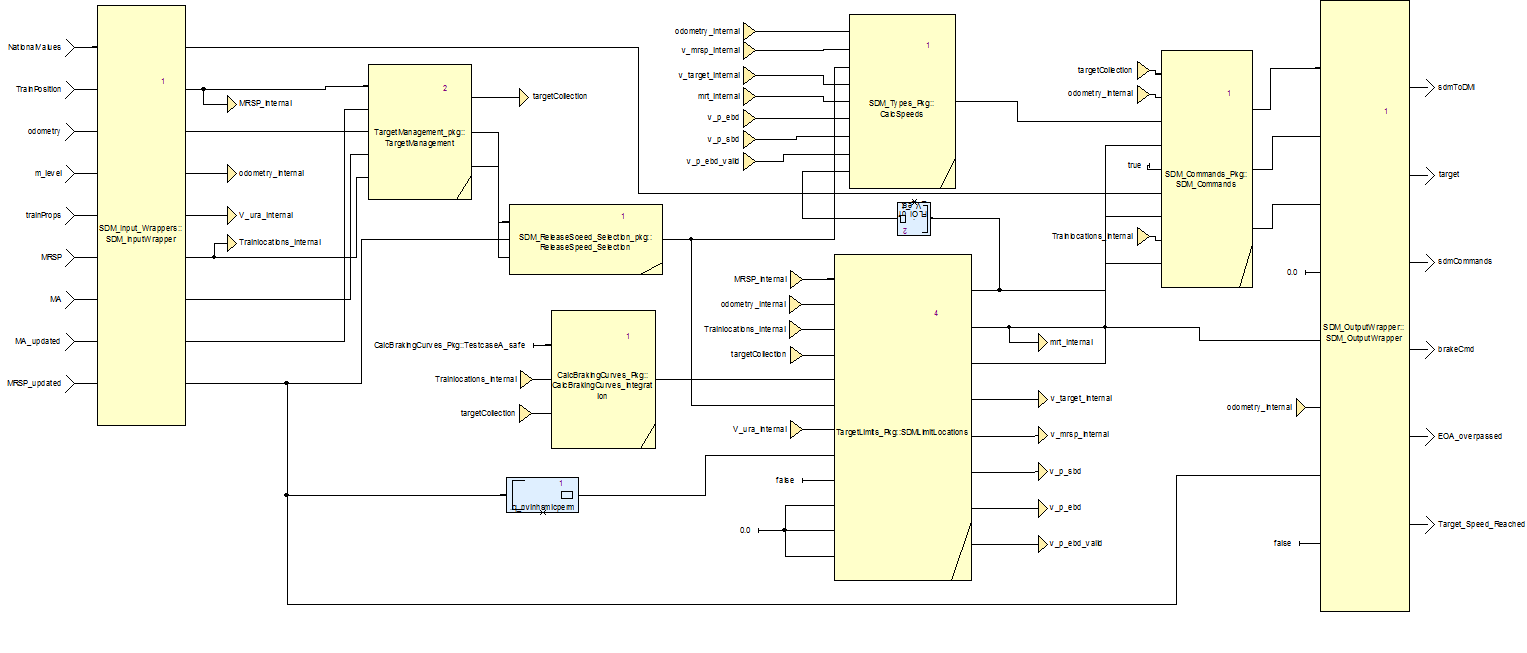
\includegraphics[width=0.95\textheight, angle=90]{../images/speedsupervision.PNG}
\caption{Structure of component ProvidePositionReport}\label{fig:ssv}
\end{figure}

The task of block ``Train Supervision'' is to monitor the speed of the train and the train location and as such to ensure that the speed remains within the given speed and distance limits. This block is mainly based on \cite[Chapt.~3.13]{subset-026}.

The block ``Train Supervision'' takes as input (1) movement related information such as train speed, train position and acceleration, (2) train related information such as brake information and train length, and (3) track related information such as speed and distance limits and national values.

Based on this information a list of targets is calculated and, for each such target, the speed the train should have. Braking curves calculate at which location at the track the train has to accelerate and to perform the brake, respectively. These calculations lead to commands being sent to the driver and the brake system.

The functionality is modeled using four operators, as shown in Figure~\ref{fig:ssv}, which are explained below.

The current status of the analysis of ``Train Supervision'' and a functional breakdown can be found in a separate document, \verb+SpeedSupervision_analysis.pdf+.



\subsubsection{Input}
For providing the output, the module needs different input data flows. Table \ref{tbl:speedsupervisionInput} gives an overview.

\begin{table}[H]
  \begin{tabular}{| c | l | l | l | l |}
    \hline
    \textbf{Index} & \textbf{Input name} & \textbf{Input type} & \textbf{Source}\\ \hline
    0 & \texttt{MRSP} & \texttt{MRSP\_Profile\_t} & ?? \\
    1 & \texttt{MA} & \texttt{MAs\_t} & ??\\
    2 & \texttt{NationalValues} & \texttt{P3\_NationalValues\_T} & ???\\
    3 & \texttt{TrainPosition} & \texttt{trainPosition\_T} & Manage Track Data\\
    4 & \texttt{V\_ura} & \texttt{V\_internal\_Type} & ??\\
    5 & \texttt{odometry} & \texttt{odometry\_T} & Odometry\\
    6 & \texttt{m\_level} & \texttt{M\_LEVEL} & Mode and Level\\
    7 & \texttt{trainProps} & \texttt{trainProperties\_T} & Database\\
    8 & \texttt{MA\_updated} & \texttt{bool} & internal\\
		9 & \texttt{MRSP\_updated} & \texttt{bool} & internal\\
    \hline
  \end{tabular} 
  \caption{Overview of input}
  \label{tbl:speedsupervisionInput}
\end{table}

\paragraph{Input 0: \texttt{MRSP}}
This input is the most restrictive speed profile.
\paragraph{Input 1: \texttt{MA}}
This input is a movement authority.
\paragraph{Input 2: \texttt{NationalValues}}
This input is packet 3 of \cite[Chapt.~8]{subset-026}, describing the national values. 
\paragraph{Input 3: \texttt{TrainPosition}}
This input is the current train position.
\paragraph{Input 4: \texttt{V\_ura}}
This input is the speed under reading amount.
\paragraph{Input 5: \texttt{odometry}}
This input is the odometry data.
\paragraph{Input 6: \texttt{m\_level}}
This input is the current level of the train.
\paragraph{Input 7: \texttt{trainProps}}
This input is a set of train related properties.
\paragraph{Input 8: \texttt{MA\_updated}}
This flag is true if the movement authority has been updated in this clock cycle and false otherwise.
\paragraph{Input 9: \texttt{MRSP\_updated}}
This flag is true if the most restrictive speed profile has been updated in this clock cycle and false otherwise.



\subsubsection{Output}
Based on the input the block produces the following output. Table~\ref{tbl:speedsupervisionOutput} gives an overview.

\begin{table}[H]
  \begin{tabular}{| c | l | l | l |}
    \hline
    \textbf{Index} & \textbf{Output name} & \textbf{Output type}\\ \hline
    0 & \texttt{sdmToDMI} & \texttt{speedSupervisionForDMI\_T}\\
    1 & \texttt{target} & \texttt{Target\_T}\\
    2 & \texttt{sdmCommands} & \texttt{SDM\_Commands\_T}\\
    3 & \texttt{brakeCmd} & \texttt{Brake\_command\_T}\\
    4 & \texttt{EOA\_overpassed} & \texttt{bool}\\
    5 & \texttt{Target\_Speed\_Reached} & \texttt{bool}\\
    \hline
  \end{tabular} 
  \caption{Overview of output}
  \label{tbl:speedsupervisionOutput}
\end{table}

\paragraph{Output 0: \texttt{sdmToDMI}}
This output contains information about different speeds and positions, on the one hand and the current supervision status, on the other hand. This information shall be displayed to the driver.
\paragraph{Output 1: \texttt{target}}
This output is the most restrictive displayed target (MRDT).
\paragraph{Output 2: \texttt{sdmCommands}}
This output gives some intermediate results of operator SDM\_Commands. It is currently used for test purposes only.
\paragraph{Output 3: \texttt{brakeCmd}}
This output is the brake command, indicating whether performing the service brake or the emergency brake have been commanded.
\paragraph{Output 4: \texttt{EOA\_overpassed}}
This output is true if the end of authority has been overpassed and false otherwise.
\paragraph{Output 5: \texttt{Target\_Speed\_Reached}}
This output is true if the current speed is greater than or equal the target speed and false otherwise.



\subsubsection{SDM\_InputWrapper in Train Supervision}

\paragraph{Reference to the SRS or other Requirements (or other requirements)}
\begin{itemize}
	\item \cite[Chapt.~3.13]{subset-026}: Speed and distance monitoring 
\end{itemize}

\paragraph{Short description of the functionality}
The motivation for this operator is to convert all inputs of block ``Speed Supervision'' that contain information about length, speed, distance, and acceleration defined as integer into real to allow for highest precision in the calculations. In addition, to ease the modeling, inside block ``Speed Supervision'' only units meters, seconds, and meters per square second are used.

\paragraph{Interface}

\paragraph{Functional Design Description}
This operator forwards input messages, takes data from complex data types or transforms inputs messages into an internal type thereby converting int to real.
  
\paragraph{Reference to the Scade Model}
\textbf{only in special case or link to the Scade model}

\subsubsection{TargetManagement in Train Supervision} \marginpar{Ben}
\paragraph{Reference to the SRS or other Requirements (or other requirements)}
\begin{itemize}
	\item \cite[Chapt.~3.13.8.2]{subset-026}: Determination of the supervised targets 
\end{itemize}

\paragraph{Short description of the functionality}
This operator calculates/updates the list of targets to be supervised by the block ``Train Supervision''. Taking the current movement authority and the most restrictive speed profile as an input, the operator outputs a list of locations corresponding to the most restrictive speed profile, a list of locations corresponding to a limit of authority, the location of an end of authority, or the location of supervised location.
  
\paragraph{Interface}

\paragraph{Functional Design Description}

\paragraph{Reference to the Scade Model}
\textbf{only in special case or link to the Scade model}

\subsubsection{CalcBrakingCurves\_Integration in Train Supervision} \marginpar{Ben}
\paragraph{Reference to the SRS or other Requirements (or other requirements)}
\begin{itemize}
	\item \cite[Chapt.~3.13.8.3]{subset-026}: Emergency Brake Deceleration curves (EBD)
	%
	\item \cite[Chapt.~3.13.8.4]{subset-026}: Service Brake Deceleration curves (SBD)
	%
	\item \cite[Chapt.~3.13.8.5]{subset-026}: Guidance curves (GUI)
\end{itemize}
\paragraph{Short description of the functionality}
For each type of target a certain braking curve has to be calculated. This curve enables us, given a target speed, to calculate the destination when this speed will be reached. In addition, given a target location, also the speed of the train at this location can be calculated. 
\paragraph{Interface}
\paragraph{Functional Design Description}
Some details about how the curves are calculated \dots

Currently, the model supports the calculation of the following braking curves:
\begin{itemize}
	\item the Emergency Brake Deceleration curve for the most restrictive speed profile,
	%
	\item the Emergency Brake Deceleration curve for the limit of authority,
	%
	\item the Emergency Brake Deceleration curve for the end of authority, and
	%
	\item the Service Brake Deceleration curve for the end of authority
\end{itemize}
\paragraph{Reference to the Scade Model}
\textbf{only in special case or link to the Scade model}

\subsubsection{SDMLimitLocations in Train Supervision} \marginpar{Tho}
\paragraph{Reference to the SRS or other Requirements (or other requirements)}
\begin{itemize}
	\item \cite[Chapt.~3.13.9]{subset-026}: Supervision Limits 
\end{itemize}

\paragraph{Short description of the functionality}
This operator calculates the various locations needed to determine the speed and distance monitoring commands.

\paragraph{Interface}
\paragraph{Functional Design Description}
\paragraph{Reference to the Scade Model}
\textbf{only in special case or link to the Scade model}

\subsubsection{CalcSpeeds in Train Supervision}
\paragraph{Reference to the SRS or other Requirements (or other requirements)}
\begin{itemize}
	\item \cite[Chapt.~3.13.9]{subset-026}: Supervision Limits 
\end{itemize}
\paragraph{Short description of the functionality}
This operator calculates the various speeds needed to determine the speed and distance monitoring commands.
\paragraph{Interface}
\paragraph{Functional Design Description}
This operator will be integrated into other operators in the next iteration.
\paragraph{Reference to the Scade Model}
\textbf{only in special case or link to the Scade model}

\subsubsection{SDM\_Commands in Train Supervision}
\paragraph{Reference to the SRS or other Requirements (or other requirements)}
\begin{itemize}
	\item \cite[Chapt.~3.13.10]{subset-026}: Speed and distance monitoring commands 
\end{itemize}
\paragraph{Short description of the functionality}
This operator models the speed and distance monitoring commands. More precisely, it triggers the service or emergency brake and outputs the current supervision status of the OBU together with information on speeds and locations to the driver.
\paragraph{Interface}
\paragraph{Functional Design Description}
The OBU can be in any of three types of speed and distance monitoring modes: ceiling speed monitoring, release speed monitoring and target speed monitoring. We use a state machine to model the switching between the three modes: each state models a mode and a transition between to states is enabled if the condition two switch between the two corresponding modes is evaluated to true. In each mode, the OBU can be in up to five different supervision stati. The behavior of changing from one status to another is also modeled as a state machine. As a result, the model is a hierarchical state machine.
\paragraph{Reference to the Scade Model}
\textbf{only in special case or link to the Scade model}

\subsubsection{SDM\_OutputWrapper in Train Supervision}
\paragraph{Reference to the SRS or other Requirements (or other requirements)}
\begin{itemize}
	\item \cite[Chapt.~3.13]{subset-026}: Speed and distance monitoring 
\end{itemize}

\paragraph{Short description of the functionality}
This operator is the counterpart to operator SDM\_OutputWrapper---that is, it converts all internal outputs of block ``Speed Supervision'' that contain information about length, speed, distance, and acceleration defined as real into int, such that all other blocks can stick to their types and also performs the calculation into units used by the environment.

\paragraph{Interface}

\paragraph{Functional Design Description}
This operator forwards input messages and transforms inputs messages into an internal type thereby converting real to int.
  
\paragraph{Reference to the Scade Model}
\textbf{only in special case or link to the Scade model}